\chapter{การเรียงลำดับและการค้นหา (Sorting \& Searching)}
\section{การเรียงลำดับ (Sorting)}

การเรียงลำดับแต่ละชนิดมีความแตกต่างกันที่ time complexity และ space complexity จึงควรที่จะเข้าใจแนวคิดของการเรียงลำดับแต่ละชนิด

\begin{figure}[h!]
	\centering
	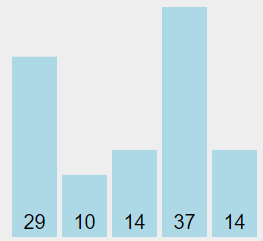
\includegraphics[width=6cm]{images/bubble_sort_start}
	\caption{ตัวอย่างอาเรย์ที่ใช้ในการเรียงลำดับ}
    \label{fig:bubble_sort_start}
\end{figure}

\subsection{การเรียงลำดับแบบฟอง (Bubble Sort)}

\begin{lstlisting}
void bubbleSort(int n){
	for (int round = 1; round <= n; round++){
		for (int idx = 0; idx < n-1; idx++){
			if (number[idx] > number[idx + 1]){
				swap(number[idx], number[idx + 1]);
			}
		}
	}
}
\end{lstlisting}

หลักการทำงาน คือ พิจารณา $a_i$ เมื่อ $0 \leq i < n-1$ หาก $a_i$ มีค่ามากกว่า $a_{i+1}$ แล้ว ให้สลับ $a_i$ และ  $a_{i+1}$ เมื่อพิจารณา $a_i$ ครบทุกจำนวนแล้วจะรับประกันได้ว่าจำนวนสุดท้ายจะมีค่ามากที่สุดอย่างแน่นอน การเรียงลำดับนี้จึงต้องทำซำ้ทั้งหมด $n$ ครั้ง เพื่อรับประกันว่าทุกจำนวนจะเรียงลำดับอย่างถูกต้อง ทำให้ใช้เวลาการทำงาน $O(n^2)$ และใช้หน่วยความจำ $O(n)$

\begin{figure}[h!]
	\centering
    \begin{subfigure}{.5\textwidth}
    	\centering
        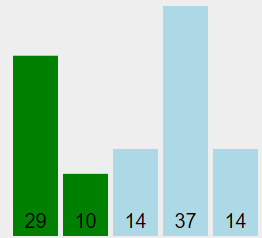
\includegraphics[width=5cm]{images/bubble_sort_1-2}
        \caption{พิจารณา $a_i$ และ $a_{i+1}$ เมื่อ $i=0$}
        \label{fig:bubble_sort_1-2}
    \end{subfigure}%
    \begin{subfigure}{.5\textwidth}
    	\centering
        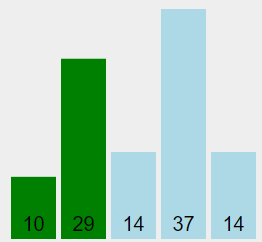
\includegraphics[width=5cm]{images/bubble_sort_1-2-swap}
        \caption{สลับ $a_i$ และ $a_{i+1}$ เมื่อ $i=0$}
        \label{fig:bubble_sort_1-2-swap}
    \end{subfigure}
    \caption{ตัวอย่างการทำงานเมื่อ $i=0$}
    \label{fig:bubble_sort_round-1-0}
\end{figure}

\begin{figure}[h!]
	\centering
    \begin{subfigure}{.5\textwidth}
    	\centering
        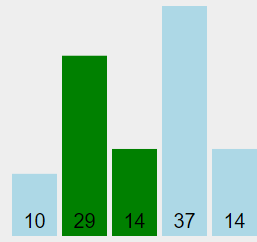
\includegraphics[width=5cm]{images/bubble_sort_2-3}
        \caption{พิจารณา $a_i$ และ $a_{i+1}$ เมื่อ $i=1$}
        \label{fig:bubble_sort_2-3}
    \end{subfigure}%
    \begin{subfigure}{.5\textwidth}
    	\centering
        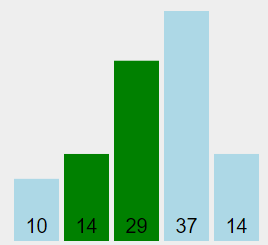
\includegraphics[width=5cm]{images/bubble_sort_2-3-swap}
        \caption{สลับ $a_i$ และ $a_{i+1}$ เมื่อ $i=1$}
        \label{fig:bubble_sort_2-3-swap}
    \end{subfigure}
    \caption{ตัวอย่างการทำงานเมื่อ $i=1$}
    \label{fig:bubble_sort_round-1-1}
\end{figure}

\begin{figure}[h!]
	\centering
    \begin{subfigure}{.5\textwidth}
    	\centering
        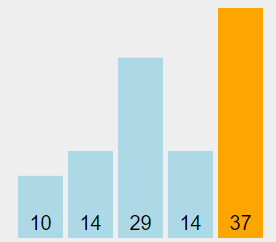
\includegraphics[width=5cm]{images/bubble_sort_round-1}
        \caption{ผลของการจัดเรียงรอบที่ 1}
        \label{fig:bubble_sort_round-1}
    \end{subfigure}%
    \begin{subfigure}{.5\textwidth}
    	\centering
        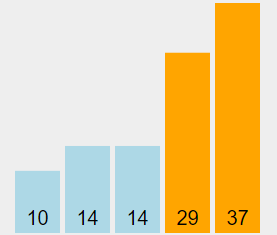
\includegraphics[width=5cm]{images/bubble_sort_round-2}
        \caption{ผลการจัดเรียงรอบที่ 2}
        \label{fig:bubble_sort_round-2}
    \end{subfigure}
    \caption{ตัวอย่างการทำงานแต่ละรอบ}
    \label{fig:bubble_sort_round-1-2}
\end{figure}

\newpage

\subsection{การเรียงลำดับแบบเลือก (Selection Sort)}

\begin{lstlisting}
void selectionSort(int n){
	for (int i = 0; i < n; i++){
		int minIndex, minValue;
		minValue = a[i];
		for (int j = i + 1; j < n; j++){
			if (minValue > a[j]){
				minValue = a[j];
				minIndex = j;
			}
		}
		swap(a[i], a[minIndex]);
	}
}
\end{lstlisting}

Selection sort มีหลักการทำงาน คือ การเลือกจำนวนที่น้อยที่สุดมาไว้ด้านหน้าของอาเรย์เรื่อยๆ จนครบทั้ง $n$ จำนวน จึงต้องใช้เวลาการทำงาน $O(n^2)$ และหน่วยความจำ $O(n)$

\begin{figure}[h!]
	\centering
    \begin{subfigure}{.5\textwidth}
    	\centering
        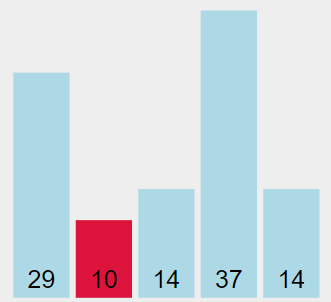
\includegraphics[width=5cm]{images/selection-sort-round-1-1}
        \caption{การเลือกจำนวนที่น้อยที่สุดรอบที่ 1}
        \label{fig:selection_sort_round-1-1}
    \end{subfigure}%
    \begin{subfigure}{.5\textwidth}
    	\centering
        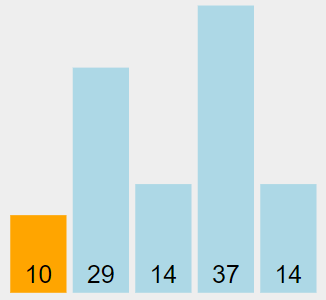
\includegraphics[width=5cm]{images/selection-sort-round-1-2}
        \caption{การนำจำนวนที่น้อยที่สุดที่ได้ในรอบที่ 1 ไปไว้ด้านหน้าสุด}
        \label{fig:selection_sort_round-1-2}
    \end{subfigure}
    \caption{การทำงานรอบที่ 1 ของ Selection sort}
    \label{fig:selection_sort_round-1}
\end{figure}

\begin{figure}[h!]
	\centering
    \begin{subfigure}{.5\textwidth}
    	\centering
        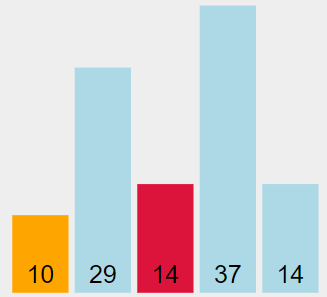
\includegraphics[width=5cm]{images/selection-sort-round-2-1}
        \caption{การเลือกจำนวนที่น้อยที่สุดรอบที่ 2}
        \label{fig:selection_sort_round-2-1}
    \end{subfigure}%
    \begin{subfigure}{.5\textwidth}
    	\centering
        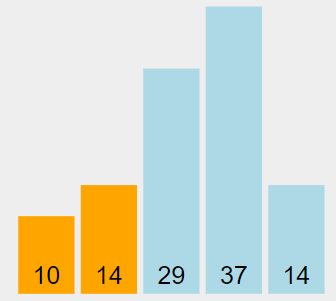
\includegraphics[width=5cm]{images/selection-sort-round-2-2}
        \caption{การนำจำนวนที่น้อยที่สุดที่ได้ในรอบที่ 2 ไปไว้ด้านหน้าต่อจากจำนวนที่เรียงแล้ว}
        \label{fig:selection_sort_round-2-2}
    \end{subfigure}
    \caption{การทำงานรอบที่ 2 ของ Selection sort}
    \label{fig:selection_sort_round-2}
\end{figure}

\newpage

\subsection{การเรียงลำดับแบบแทรก (Insertion Sort)}

\begin{lstlisting}
void insertionSort(int n){
	for (int i = 0; i < n; i++){
		for (int j = i - 1; j >= 0; j--){
			if (a[j] > a[j + 1]){
				swap(a[j], a[j + 1]);
			}else{
				break;
			}
		}
	}
}
\end{lstlisting}

Insertion sort มีหลักการทำงาน คือ พิจารณาทีละจำนวน และหากจำนวนนั้นไม่ได้อยู่ในตำแหน่งที่ถูกต้อง (เช่น ต้องการเรียงจากน้อยไปมาก แต่จำนวนที่กำลังพิจารณามีค่าน้อยกว่าจำนวนก่อนหน้า หมายความว่า จำนวนอยู่ผิดตำแหน่ง) ให้สลับกับจำนวนก่อนหน้าจนกว่าจะอยู่ในตำแหน่งที่ถูกต้อง

\begin{figure}[h!]
	\centering
    \begin{subfigure}{.5\textwidth}
    	\centering
        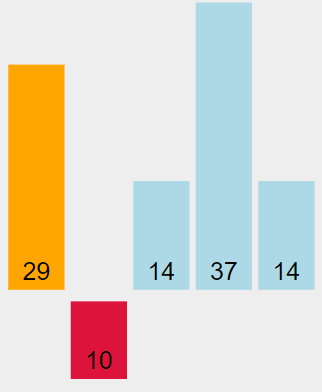
\includegraphics[width=4cm]{images/insertion_sort_round-2-1}
        \caption{พิจารณาจำนวนที่ 2 (เลข 10)}
        \label{fig:insertion_sort_round-2-1}
    \end{subfigure}%
    \begin{subfigure}{.5\textwidth}
    	\centering
        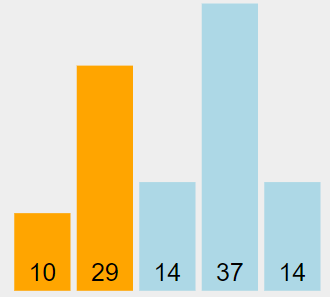
\includegraphics[width=4cm]{images/insertion_sort_round-2-2}
        \caption{แทรกเลข 10 เข้าไปหน้าเลข 29}
        \label{fig:insertion_sort_round-2-2}
    \end{subfigure}
    \caption{ตัวอย่างการทำงานรอบที่ 2 ของ Insertion sort}
    \label{fig:insertion_sort_round-2}
\end{figure}

\begin{figure}[h!]
	\centering
    \begin{subfigure}{.5\textwidth}
    	\centering
        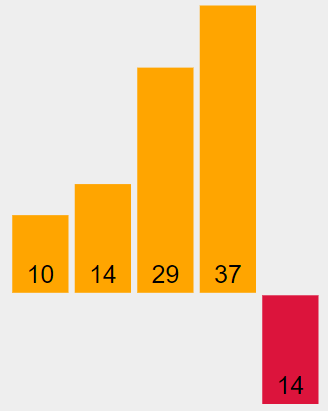
\includegraphics[width=4cm]{images/insertion_sort_round-5-1}
        \caption{พิจารณาจำนวนที่ 5 (เลข 14)}
        \label{fig:insertion_sort_round-5-1}
    \end{subfigure}%
    \begin{subfigure}{.5\textwidth}
    	\centering
        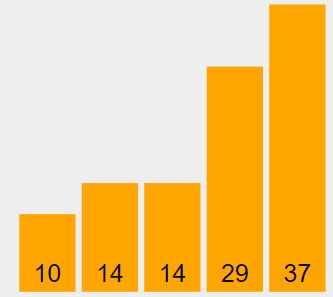
\includegraphics[width=4cm]{images/insertion_sort_round-5-2}
        \caption{แทรกเลข 14 เข้าไปหน้าเลข 29}
        \label{fig:insertion_sort_round-2-2}
    \end{subfigure}
    \caption{ตัวอย่างการทำงานรอบที่ 5 ของ Insertion sort}
    \label{fig:insertion_sort_round-2}
\end{figure}

\subsection{การเรียงลำดับแบบผสาน (Merge Sort)}

Merge Sort เป็นกระบวนการคิดแบบแบ่งแยกและเอาชนะ (Divide and Conquer algorithm) กล่าวคือ มีการแบ่งข้อมูลออกเป็น 2 ส่วนจากนั้นจึงเรียกตัวเองซำ้แบ่งข้อมูลไปเรื่อยๆ แล้วจึงนำข้อมูลแต่ละส่วนมาพิจารณาเรียงลำดับกันจากกลุ่มเล็กๆ เป็นกลุ่มใหญ่ โดยมีเวลาการทำงาน $O(n log(n))$

\begin{figure}[h!]
	\centering
    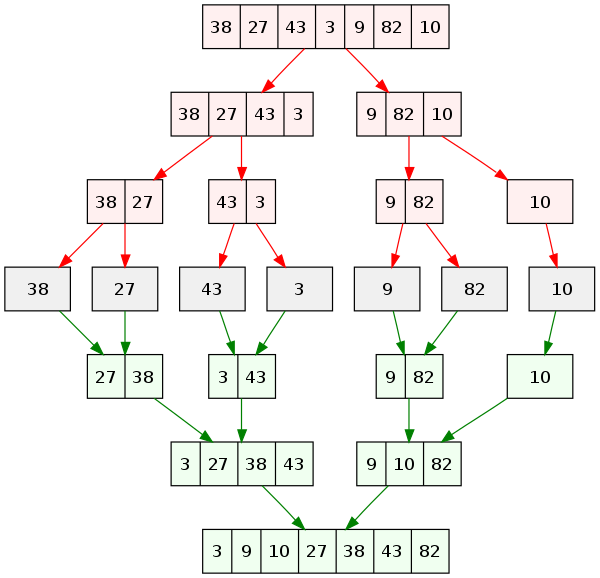
\includegraphics[width=13cm]{images/merge-sort}
    \caption{การทำงานโดยภาพรวมของ Merge Sort}
    \label{fig:merge-sort}
\end{figure}

\newpage

\begin{lstlisting}
void mergeSort(int l, int r){
	if (l == r)
		return;
	int mid = (l + r) / 2;
	mergeSort(l, mid), mergeSort(mid + 1, r);
	int i = l, j = mid + 1, k = l;
	while (i <= mid && j <= r){
		if (a[i] <= a[j])
			temp[k++] = a[i++];
		else
			temp[k++] = a[j++];
	}
	while (i <= mid)
		temp[k++] = a[i++];
	while (j <= r)
		temp[k++] = a[j++];
	for (int k = l; k <= r; k++)
		a[k] = temp[k];
}
\end{lstlisting}

\section{การค้นหา (Searching)}
\subsection{การค้นหาแบบลำดับ (Sequential Search)}

Sequential search เป้นการค้นหาโดยทั่วไป คือเริ่มตรวจสอบจากสมาชิกตัวแรกไปจนถึงตัวสุดท้ายของอาเรย์ กรณีที่แย่ที่สุดคือต้องตรวจสอบสมาชิกทุกตัวในอาเรย์ จึงใช้เวลาการทำงาน $O(n)$

\begin{figure}[h!]
	\centering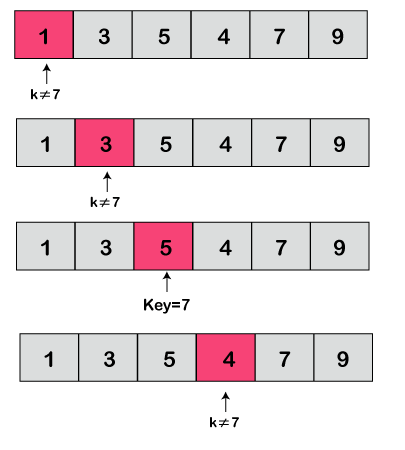
\includegraphics[width=6cm]{images/sequential_search}
    \caption{ตัวอย่างการค้นหาแบบลำดับ}
    \label{fig:sequential_search}
\end{figure}

\newpage

\begin{lstlisting}
int sequentialSearch(int n, int target){
	for (int i = 0; i < n; i++){
		if (a[i] == target){
			return i;
		}
	}
	return -1;
}
\end{lstlisting}

\subsection{การค้นหาแบบทวิภาค (Binary Search)}

Binary search เป็นเทคนิคการค้นหาที่รวดเร็วกว่า Sequential search แต่ก็แลกมาด้วยเงื่อนไขที่ว่าข้อมูลต้องเรียงลำดับมาก่อนแล้ว จึงจะสามารถใช้ได้

\begin{figure}[h!]
	\centering
    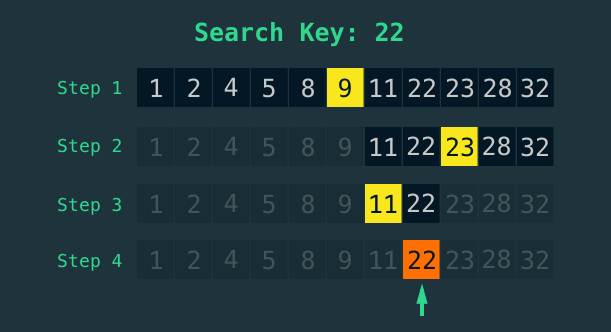
\includegraphics[width=13cm]{images/binary-search}
    \caption{ตัวอย่างการทำงานของ Binary search}
    \label{fig:binary_search}
\end{figure}

แนวคิดของ Binary search คือการตรวจสอบข้อมูลตรงกลางของช่วงที่สนใจเพื่อพิจารณาว่าแนวโน้มของข้อมูลที่ต้องการค้นหาอยู่ในช่วงใด และทำซำ้ไปเรื่อยๆ จนกว่าจะได้ข้อสรุปอย่างแน่นอน เช่น มีอาเรย์ของจำนวนเต็ม $n$ จำนวนที่เรียงลำดับจากน้อยไปหามากอยู่ (เรียกตำแหน่งแรกเป็นตำแหน่งที่ 1 และตำแหน่งสุดท้ายเป็นตำแหน่งที่ $n$)จึงพิจารณาจำนวนที่อยู่ตำแหน่ง $\frac{n}{2}$ ว่ามีค่ามากหรือน้อยกว่าจำนวนที่ต้องการหา หากมากกว่า แสดงว่าจำนวนที่ต้องการหาอาจจะอยู่ในช่วงตำแหน่ง 1 ถึง $\frac{n}{2}-1$ ในทางกลับกัน หากน้อยกว่า แสดงว่าจำนวนที่ต้องการหาอาจจะอยู่ในช่วงตำแหน่ง $\frac{n}{2}+1$ ถึง $n$ แทน จะเห็นได้ว่า การพิจารณานี้จะทำให้ช่วงข้อมูลที่สนใจสามารถลดลงเหลือครึ่งหนึ่งได้ทันที ทำให้เวลาการทำงานก็ลดลงไปเป็น $O(log(n))$ ด้วย

\newpage

\begin{lstlisting}
int binarySearch(int n, int target){
	int l = 1, r = n;
	while (l < r){
		int mid = (l + r) / 2;
		if (a[mid] == target){
			return mid;
		}else if (a[mid] > target){
			r = mid - 1;
		}else if (a[mid] < target){
			l = mid + 1;
		}
	}
	return -1;
}
\end{lstlisting}

นอกจากนี้ ยังมี STL สำหรับ Binary Search เพื่อช่วยให้เขียนโปรแกรมได้รวดเร็วขึ้นอย่าง \texttt{lower\_bound} และ \texttt{upper\_bound} โดยจะต้องระบุตำแหน่งแรกที่ต้องการเริ่มค้นหา, ตำแหน่งสุดท้ายที่ต้องการค้นหา, และข้อมูลที่ต้องการค้นหา

เช่น ต้องการค้นหาภายในอาเรย์ของจำนวนเต็มชื่อว่า $number$ ตั้งแต่ตำแหน่งที่ 1 ถึงตำแหน่งที่ $n$ โดยต้องการค้นหาเลข 10 จะเรียกใช้แบบนี้
\begin{itemize}
\item lower\_bound(number + 1, number + n, 10);
\item upper\_bound(number + 1, number + n, 10);
\end{itemize}

\noindent และทั้ง 2 ฟังก์ชั่นมีความแตกต่างกันเล็กน้อยดังนี้
\begin{itemize}
\item หากเรียกใช้ lower\_bound
\begin{itemize}
\item มีข้อมูลที่ต้องการค้นหาอยู่ในกลุ่มข้อมูลทั้งหมด จะคืนค่าตำแหน่งที่พบตำแหน่งแรกสุด เช่น มีอาเรย์ 2 2 3 4 5 อยู่ และต้องการค้นหาเลข 2 จะคืนค่าตำแหน่งที่ 1 ออกมา
\item ไม่มีข้อมูลที่ต้องการค้นหา จะคืนค่าตำแหน่งถัดไปที่ใกล้เคียงที่สุด เช่น มีอาเรย์ 2 2 3 6 ต้องการค้นหาเลข 4 จะคืนค่าตำแหน่งที่ 4 ออกมา
\end{itemize}
\item หากเรียกใช้ upper\_bound ไม่ว่าจะมี/ไม่มีข้อมูลที่ต้องการค้นหา จะคืนค่าตำแหน่งถัดไปที่ใกล้เคียงที่สุด
\end{itemize}
